% ============================================================================
% Multi-Target Stock Prediction Using Ensemble Deep Learning
% Master's Thesis Presentation - Beamer LaTeX
% ============================================================================
\documentclass[aspectratio=43,11pt]{beamer}

% ================== THEME AND COLORS ==================
\usetheme{Madrid}
\usecolortheme{whale}

% Custom Colors
\definecolor{primaryblue}{RGB}{0,51,102}
\definecolor{accentorange}{RGB}{255,128,0}
\definecolor{lightgray}{RGB}{240,240,240}
\definecolor{successgreen}{RGB}{40,167,69}
\definecolor{warningred}{RGB}{220,53,69}

\setbeamercolor{palette primary}{bg=primaryblue,fg=white}
\setbeamercolor{palette secondary}{bg=primaryblue!80,fg=white}
\setbeamercolor{palette tertiary}{bg=primaryblue!60,fg=white}
\setbeamercolor{structure}{fg=primaryblue}
\setbeamercolor{title}{fg=white,bg=primaryblue}
\setbeamercolor{frametitle}{fg=white,bg=primaryblue}
\setbeamercolor{block title}{bg=primaryblue,fg=white}
\setbeamercolor{block body}{bg=lightgray}
\setbeamercolor{block title example}{bg=successgreen,fg=white}
\setbeamercolor{block title alerted}{bg=warningred,fg=white}

% ================== PACKAGES ==================
\usepackage{graphicx}
\usepackage{booktabs}
\usepackage{tabularx}
\usepackage{adjustbox}
\usepackage{amsmath,amssymb}
\usepackage{tikz}
\usepackage{multirow}
\usepackage{hyperref}
\hypersetup{pdfpagemode=FullScreen,pdfpagelayout=SinglePage}
\usepackage{xcolor}
\usepackage{colortbl}

\usetikzlibrary{shapes,arrows,positioning,calc,fit,backgrounds}

% ================== SETTINGS ==================
\setbeamertemplate{navigation symbols}{}
\setbeamertemplate{footline}[frame number]
\setbeamertemplate{itemize items}[circle]
\setbeamertemplate{enumerate items}[default]

% Graphics path
\graphicspath{{../evaluation_results/plots/}{images/}}

% ================== TITLE INFO ==================
\title[Multi-Target Stock Prediction]{\small\textbf{Development of Positional Trading Strategy Using Deep Learning and Its Training, Testing, and Implementation on a Real-Time Platform Using API}}
\subtitle{End Sem Project Phase - 1 Presentation}
\author{Presented by: Vishwam Shah\\[0.2cm]\small Under the Guidance of: Dr. Jigarkumar Shah}
\institute{Pandit Deendayal Energy University\\School of Technology}
\date{December 2025}
\titlegraphic{\includegraphics[height=1.2cm]{pdeulogo.png}}

% ============================================================================
% DOCUMENT START
% ============================================================================
\begin{document}

% ================== TITLE SLIDE ==================
\begin{frame}
    \titlepage
\end{frame}

% ================== OUTLINE ==================
\begin{frame}{Presentation Outline}
    \tableofcontents
\end{frame}

% ============================================================================
\section{Introduction \& Motivation}
% ============================================================================

\begin{frame}{Research Motivation}
    \begin{columns}[T]
        \begin{column}{0.48\textwidth}
            \textbf{The Challenge:}
            \begin{itemize}
                \item Stock markets are highly volatile and non-linear
                \item Traditional models fail to capture complex patterns
                \item Single-target predictions miss critical information
                \item Need for robust, multi-target forecasting
            \end{itemize}
            
        \end{column}
        \begin{column}{0.48\textwidth}
            \begin{block}{Key Statistics}
                \begin{itemize}
                    \item \textbf{106} NSE Stocks Analyzed
                    \item \textbf{244} Engineered Features
                    \item \textbf{4} Prediction Targets
                    \item \textbf{10} Years of Data (2015-2025)
                    \item \textbf{64.7M} Total Data Points
                \end{itemize}
            \end{block}
            
            \begin{alertblock}{Main Achievement}
                \textbf{68.28\%} Direction Accuracy\\
                (36\% above random baseline)
            \end{alertblock}
        \end{column}
    \end{columns}
\end{frame}

% ============================================================================
\section{Dataset \& Stock Selection}
% ============================================================================

\begin{frame}{Stock Universe: 106 NSE Stocks Across 11 Sectors}
    \begin{center}
    \small
    \adjustbox{max width=\textwidth}{
    \begin{tabular}{lcp{5.5cm}}
        \toprule
        \textbf{Sector} & \textbf{Count} & \textbf{Representative Stocks} \\
        \midrule
        Banking & 12 & HDFCBANK, ICICIBANK, SBIN, AXISBANK \\
        Information Technology & 10 & TCS, INFY, WIPRO, HCLTECH, TECHM \\
        Pharmaceuticals & 9 & SUNPHARMA, DRREDDY, CIPLA, LUPIN \\
        Automotive & 9 & MARUTI, M\&M, TATAMOTORS, BAJAJ-AUTO \\
        Energy \& Power & 11 & RELIANCE, ONGC, BPCL, NTPC, TATAPOWER \\
        Metals & 9 & TATASTEEL, JSWSTEEL, HINDALCO, VEDL \\
        Consumer Goods & 11 & HINDUNILVR, ITC, BRITANNIA, DABUR \\
        Construction & 6 & LT, DLF, GODREJPROP, OBEROIRLTY \\
        Cement & 6 & ULTRACEMCO, SHREECEM, AMBUJACEM, ACC \\
        Telecom & 3 & BHARTIARTL, IDEA, TATACOMM \\
        Others & 20 & TITAN, ASIANPAINT, BAJFINANCE, ADANIENT \\
        \midrule
        \textbf{Total} & \textbf{106} & \\
        \bottomrule
    \end{tabular}
    }
    \end{center}
    
    \vspace{0.2cm}
    \textbf{Selection Criteria:} Highest to lowest market cap coverage (diverse representation) $\bullet$ Market Cap $>$ INR 5,000 Cr $\bullet$ Complete 10-year data availability
\end{frame}

\begin{frame}{Data Characteristics}
    \begin{columns}[T]
        \begin{column}{0.48\textwidth}
            \begin{block}{Data Sources}
                \begin{itemize}
                    \item \textbf{Yahoo Finance:} OHLCV Data (via yfinance library)
                    \item \textbf{Market Indices:} NIFTY50, BANKNIFTY, India VIX
                    \item \textbf{Sector Indices:} Bank, IT, Pharma, Auto, etc.
                    \item \textbf{Currency:} USD/INR Exchange Rate
                \end{itemize}
            \end{block}
            
            \begin{block}{Data Pipeline}
                \begin{enumerate}
                    \item Raw OHLCV data collection
                    \item Missing value imputation
                    \item Outlier clipping (1st-99th pctl)
                    \item Feature engineering (244)
                \end{enumerate}
            \end{block}
        \end{column}
        \begin{column}{0.48\textwidth}
            \begin{block}{Temporal Split (Walk-Forward)}
                \begin{center}
                \begin{tabular}{lcc}
                    \toprule
                    \textbf{Period} & \textbf{\%} & \textbf{Years} \\
                    \midrule
                    Training & 60\% & 2015-2020 \\
                    Validation & 20\% & 2020-2022 \\
                    Testing & 20\% & 2022-2025 \\
                    \bottomrule
                \end{tabular}
                \end{center}
            \end{block}
            
            \begin{exampleblock}{Why Walk-Forward?}
                \begin{itemize}
                    \item No lookahead bias
                    \item Mimics real trading
                    \item Temporal causality preserved
                    \item Realistic performance estimation
                \end{itemize}
            \end{exampleblock}
        \end{column}
    \end{columns}
\end{frame}

% ============================================================================
\section{Feature Engineering (244 Features)}
% ============================================================================

\begin{frame}{Feature Engineering Framework: 244 Total Features}
    \begin{center}
    \small
    \adjustbox{max width=\textwidth}{
    \begin{tabular}{lcp{6cm}}
        \toprule
        \textbf{Category} & \textbf{Count} & \textbf{Key Features} \\
        \midrule
        Technical Indicators & 87 & SMA, EMA, MACD, RSI, Bollinger Bands, ATR, ADX, Stochastic \\
        Price Features & 24 & Returns (1d, 5d, 20d), Log returns, Price ratios, VWAP \\
        Volatility Indicators & 18 & Historical volatility, Parkinson, Garman-Klass, ATR-based \\
        Volume Analysis & 22 & Volume ratios, OBV, CMF, Volume RSI, VWAP deviations \\
        Market Regime & 31 & Trend strength, Support/resistance, Breakout detection \\
        Temporal Features & 12 & Day of week, Month, Quarter, Trading patterns \\
        Sentiment Features & 15 & News sentiment, Sentiment momentum, Social indicators \\
        Interaction Features & 35 & Price-volume, RSI-MACD divergence, Multi-timeframe \\
        \midrule
        \textbf{TOTAL} & \textbf{244} & \\
        \bottomrule
    \end{tabular}
    }
    \end{center}
    
    \vspace{0.2cm}
    \textbf{Feature Selection:} Correlation analysis ($\rho > 0.95$ removed) $\rightarrow$ RFE with XGBoost $\rightarrow$ Domain validation
    
    \vspace{0.2cm}
    \footnotesize\textbf{Full Feature List:} \textcolor{primaryblue}{\url{https://docs.google.com/spreadsheets/d/1HlD8WWPD7ANzqNEcoHR1YztSjAFUIJ7L}}
\end{frame}

\begin{frame}{Key Technical Indicators Used}
    \begin{columns}
        \begin{column}{0.33\textwidth}
            \begin{block}{Momentum (30+)}
                \begin{itemize}
                    \item RSI (14-day)
                    \item MACD (12,26,9)
                    \item Stochastic Oscillator
                    \item Rate of Change (ROC)
                    \item Williams \%R
                    \item CCI
                \end{itemize}
            \end{block}
        \end{column}
        \begin{column}{0.33\textwidth}
            \begin{block}{Trend (25+)}
                \begin{itemize}
                    \item SMA (10, 20, 50, 200)
                    \item EMA (10, 20, 50)
                    \item ADX
                    \item Aroon Indicator
                    \item Ichimoku Cloud
                    \item Parabolic SAR
                \end{itemize}
            \end{block}
        \end{column}
        \begin{column}{0.33\textwidth}
            \begin{block}{Volatility (18+)}
                \begin{itemize}
                    \item Bollinger Bands
                    \item ATR (14-day)
                    \item Keltner Channel
                    \item Historical Vol
                    \item Parkinson Vol
                    \item Garman-Klass
                \end{itemize}
            \end{block}
        \end{column}
    \end{columns}
    
    \vspace{0.5cm}
    \begin{alertblock}{Feature Engineering Impact}
        Accuracy improved from \textbf{50\%} (baseline 72 features) to \textbf{68.28\%} (244 features) --- \textbf{+18.28 percentage points!}
    \end{alertblock}
\end{frame}

% ============================================================================
\section{Multi-Target Prediction Framework}
% ============================================================================

\begin{frame}{Four Prediction Targets}
    \begin{columns}[T]
        \begin{column}{0.48\textwidth}
            \begin{block}{Target 1: Direction (Classification)}
                \textbf{Formula:} $\text{Up if } \log\left(\frac{C_{t+1}}{C_t}\right) > 0$
                
                Binary classification: Up / Down movement
            \end{block}
            
            \begin{block}{Target 2: Close Return (Regression)}
                \textbf{Formula:} $r_{close} = \log\left(\frac{C_{t+1}}{C_t}\right)$
                
                Next-day closing price change
            \end{block}
        \end{column}
        \begin{column}{0.48\textwidth}
            \begin{block}{Target 3: High Return (Regression)}
                \textbf{Formula:} $r_{high} = \log\left(\frac{H_{t+1}}{O_{t+1}}\right)$
                
                Maximum potential profit from open
            \end{block}
            
            \begin{block}{Target 4: Low Return (Regression)}
                \textbf{Formula:} $r_{low} = \log\left(\frac{L_{t+1}}{O_{t+1}}\right)$
                
                Maximum potential loss (stop-loss level)
            \end{block}
        \end{column}
    \end{columns}
    
    \vspace{0.2cm}
    \begin{exampleblock}{Multi-Task Benefits}
        \small
        Shared representations $\rightarrow$ better generalization; Target correlation $\rightarrow$ risk assessment
    \end{exampleblock}
\end{frame}

% ============================================================================
\section{Model Architecture}
% ============================================================================

\begin{frame}{Individual Models Used}
    \begin{columns}[T]
        \begin{column}{0.32\textwidth}
            \begin{block}{XGBoost}
                \centering
                \textbf{Gradient Boosting}
                \vspace{0.2cm}
                \begin{itemize}\footnotesize
                    \item Tree-based model
                    \item Sequential error correction
                    \item Feature importance
                    \item L1/L2 regularization
                \end{itemize}
            \end{block}
        \end{column}
        \begin{column}{0.32\textwidth}
            \begin{block}{LSTM}
                \centering
                \textbf{Long Short-Term Memory}
                \vspace{0.2cm}
                \begin{itemize}\footnotesize
                    \item Recurrent neural network
                    \item Memory cells for sequences
                    \item Captures long dependencies
                    \item Gate mechanisms
                \end{itemize}
            \end{block}
        \end{column}
        \begin{column}{0.32\textwidth}
            \begin{block}{GRU}
                \centering
                \textbf{Gated Recurrent Unit}
                \vspace{0.2cm}
                \begin{itemize}\footnotesize
                    \item Simplified LSTM variant
                    \item Fewer parameters
                    \item Reset \& update gates
                    \item Faster training
                \end{itemize}
            \end{block}
        \end{column}
    \end{columns}
    
    \vspace{0.5cm}
    \begin{alertblock}{Model Selection Rationale}
        \centering
        XGBoost for tabular feature learning $\bullet$ LSTM/GRU for sequential pattern recognition $\bullet$ Complementary strengths
    \end{alertblock}
\end{frame}

\begin{frame}{Ensemble Architecture (Stacking)}
    \begin{center}
    \resizebox{0.9\textwidth}{!}{%
    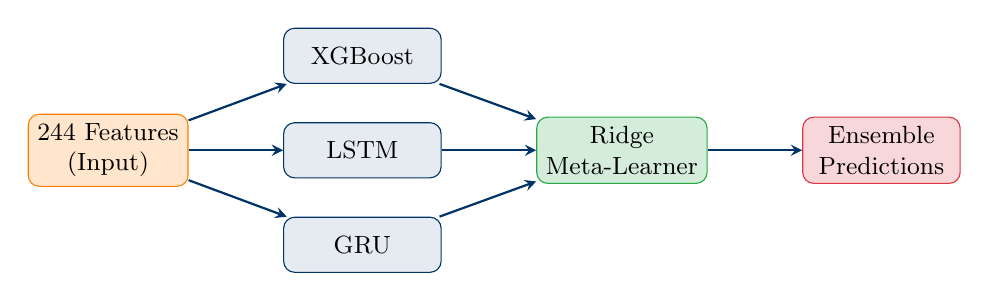
\begin{tikzpicture}[
        node distance=1cm,
        box/.style={rectangle, draw=primaryblue, fill=primaryblue!10, minimum width=2cm, minimum height=0.7cm, align=center, rounded corners, font=\small},
        arrow/.style={->, >=stealth, thick, primaryblue}
    ]
        % Input
        \node[box, fill=accentorange!20, draw=accentorange] (input) {244 Features\\(Input)};
        
        % Models
        \node[box, right=1.2cm of input, yshift=1.2cm] (xgb) {XGBoost};
        \node[box, right=1.2cm of input, yshift=0cm] (lstm) {LSTM};
        \node[box, right=1.2cm of input, yshift=-1.2cm] (gru) {GRU};
        
        % Meta-learner
        \node[box, right=1.2cm of lstm, fill=successgreen!20, draw=successgreen] (meta) {Ridge\\Meta-Learner};
        
        % Output
        \node[box, right=1.2cm of meta, fill=warningred!20, draw=warningred] (output) {Ensemble\\Predictions};
        
        % Arrows
        \draw[arrow] (input) -- (xgb);
        \draw[arrow] (input) -- (lstm);
        \draw[arrow] (input) -- (gru);
        \draw[arrow] (xgb) -- (meta);
        \draw[arrow] (lstm) -- (meta);
        \draw[arrow] (gru) -- (meta);
        \draw[arrow] (meta) -- (output);
    \end{tikzpicture}
    }%
    \end{center}
    
    \vspace{0.3cm}
    \textbf{Stacking Ensemble:} Individual models trained independently $\rightarrow$ Meta-learner combines predictions $\rightarrow$ Final weighted output
\end{frame}

\begin{frame}{Model Specifications}
    \begin{columns}[T]
        \begin{column}{0.48\textwidth}
            \begin{block}{XGBoost}
                \footnotesize
                \begin{itemize}
                    \item 200 estimators, max\_depth=5
                    \item Learning rate: 0.01
                    \item Subsample: 0.8
                    \item L2 regularization ($\lambda$=1.0)
                    \item Early stopping: 20 rounds
                \end{itemize}
            \end{block}
            \vspace{0.2cm}
            \begin{block}{LSTM}
                \footnotesize
                \begin{itemize}
                    \item 2 layers: 128 $\rightarrow$ 64 units
                    \item Dropout: 0.3
                    \item Sequence length: 10 days
                    \item Adam optimizer (lr=0.001)
                \end{itemize}
            \end{block}
        \end{column}
        \begin{column}{0.48\textwidth}
            \begin{block}{GRU}
                \footnotesize
                \begin{itemize}
                    \item 2 layers: 128 $\rightarrow$ 64 units
                    \item Similar config to LSTM
                    \item Faster training
                    \item Fewer parameters
                \end{itemize}
            \end{block}
            \vspace{0.2cm}
            \begin{block}{Ensemble (Stacking)}
                \footnotesize
                \begin{itemize}
                    \item Meta-learner: Ridge ($\alpha$=1.0)
                    \item Trained on validation predictions
                    \item Weighted combination
                    \item Best of both worlds
                \end{itemize}
            \end{block}
        \end{column}
    \end{columns}
\end{frame}

% ============================================================================
\section{Results \& Performance}
% ============================================================================

\begin{frame}{Overall Performance: 106 Stocks}
    \begin{center}
    \begin{tabular}{lccccc}
        \toprule
        \textbf{Model} & \textbf{Dir. Acc.} & \textbf{Close R\textsuperscript{2}} & \textbf{RMSE (\%)} & \textbf{MAE (\%)} & \textbf{F1} \\
        \midrule
        \rowcolor{successgreen!30}
        \textbf{Ensemble} & \textbf{68.28\%} & \textbf{0.027} & \textbf{1.37\%} & \textbf{1.01\%} & \textbf{0.702} \\
        XGBoost & 68.22\% & 0.0178 & 1.38\% & 1.02\% & 0.695 \\
        LSTM & 50.31\% & -0.003 & 1.39\% & 1.03\% & 0.669 \\
        GRU & 50.28\% & -0.003 & 1.39\% & 1.03\% & 0.669 \\
        \bottomrule
    \end{tabular}
    \end{center}
    
    \vspace{0.3cm}
    \begin{columns}[T]
        \begin{column}{0.48\textwidth}
            \begin{exampleblock}{Key Findings}
                \begin{itemize}
                    \item XGBoost: \textbf{Best on 54 stocks}
                    \item Ensemble: Close second (52 stocks)
                    \item LSTM/GRU: Near-random ($\sim$50\%)
                \end{itemize}
            \end{exampleblock}
        \end{column}
        \begin{column}{0.48\textwidth}
            \begin{alertblock}{Neural Network Challenge}
                LSTM/GRU show \textbf{overfitting}:
                \begin{itemize}
                    \item High training accuracy
                    \item Poor test generalization
                    \item Predicts majority class
                \end{itemize}
            \end{alertblock}
        \end{column}
    \end{columns}
\end{frame}

\begin{frame}{Best Model Distribution}
    \begin{columns}[T]
        \begin{column}{0.48\textwidth}
            \begin{center}
            \begin{tabular}{lcc}
                \toprule
                \textbf{Model} & \textbf{Stocks} & \textbf{\%} \\
                \midrule
                \rowcolor{successgreen!30}
                Ensemble & 58 & 54.7\% \\
                XGBoost & 46 & 43.4\% \\
                LSTM & 1 & 0.9\% \\
                GRU & 1 & 0.9\% \\
                \midrule
                \textbf{Total} & \textbf{106} & \textbf{100\%} \\
                \bottomrule
            \end{tabular}
            \end{center}
            
            \vspace{0.3cm}
            \textbf{Insight:} Ensemble wins on 58/106 stocks (54.7\%), validating the stacking approach that combines model strengths.
        \end{column}
        \begin{column}{0.48\textwidth}
            \begin{center}
            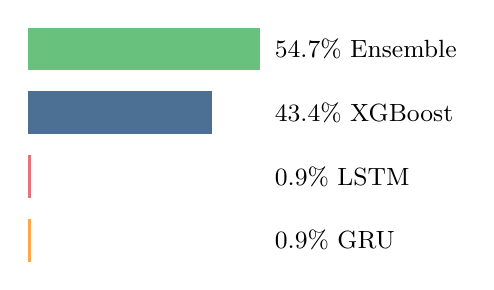
\begin{tikzpicture}[scale=0.9]
                % Bar chart
                \fill[successgreen!70] (0,0) rectangle (3.28,0.6);
                \node[right] at (3.35,0.3) {\small 54.7\% Ensemble};
                
                \fill[primaryblue!70] (0,-0.9) rectangle (2.60,0.6-0.9);
                \node[right] at (3.35,-0.6) {\small 43.4\% XGBoost};
                
                \fill[warningred!70] (0,-1.8) rectangle (0.05,0.6-1.8);
                \node[right] at (3.35,-1.5) {\small 0.9\% LSTM};
                
                \fill[accentorange!70] (0,-2.7) rectangle (0.05,0.6-2.7);
                \node[right] at (3.35,-2.4) {\small 0.9\% GRU};
            \end{tikzpicture}
            \end{center}
        \end{column}
    \end{columns}
\end{frame}

\begin{frame}{Performance by Target Variable}
    \begin{center}
    \footnotesize
    \begin{tabular}{lcccc}
        \toprule
        \textbf{Target / Metric} & \textbf{XGBoost} & \textbf{LSTM} & \textbf{GRU} & \textbf{Ensemble} \\
        \midrule
        \multicolumn{5}{c}{\textit{Close Price Return}} \\
        \midrule
        R\textsuperscript{2} Score & 0.0178 & -0.0027 & -0.0026 & \textbf{0.0270} \\
        RMSE (\%) & 1.38 & 1.39 & 1.39 & \textbf{1.37} \\
        \midrule
        \multicolumn{5}{c}{\textit{High Price Return}} \\
        \midrule
        R\textsuperscript{2} Score & -0.0412 & -0.0687 & -0.0686 & -0.0821 \\
        RMSE (\%) & \textbf{1.09} & 1.11 & 1.11 & 1.13 \\
        \midrule
        \multicolumn{5}{c}{\textit{Low Price Return}} \\
        \midrule
        R\textsuperscript{2} Score & \textbf{0.0089} & -0.0421 & -0.0419 & -0.0315 \\
        RMSE (\%) & \textbf{1.03} & 1.05 & 1.05 & 1.04 \\
        \midrule
        \multicolumn{5}{c}{\textit{Direction (Classification)}} \\
        \midrule
        Accuracy & 68.22\% & 50.31\% & 50.28\% & \textbf{68.28\%} \\
        F1-Score & 0.6954 & 0.6686 & 0.6685 & \textbf{0.7024} \\
        \bottomrule
    \end{tabular}
    \end{center}
\end{frame}

% ============================================================================
\section{Case Study: RELIANCE}
% ============================================================================

\begin{frame}{Case Study: RELIANCE Industries}
    \begin{columns}[T]
        \begin{column}{0.38\textwidth}
            \begin{block}{Stock Profile}
                \begin{itemize}
                    \item \textbf{Sector:} Energy
                    \item \textbf{Market Cap:} \#1 in India
                    \item \textbf{Volatility:} Moderate-High
                    \item \textbf{Test Samples:} 512 days
                \end{itemize}
            \end{block}
            
            \begin{center}
            \begin{tabular}{lc}
                \toprule
                \textbf{Model} & \textbf{Dir. Acc.} \\
                \midrule
                XGBoost & 71.62\% \\
                LSTM & 52.62\% \\
                GRU & 52.62\% \\
                \rowcolor{successgreen!30}
                \textbf{Ensemble} & \textbf{72.23\%} \\
                \bottomrule
            \end{tabular}
            \end{center}
        \end{column}
        \begin{column}{0.58\textwidth}
            \begin{figure}
                \includegraphics[width=\textwidth]{RELIANCE_comparison_plot.png}
                \caption{RELIANCE: Actual vs Predicted Prices}
            \end{figure}
        \end{column}
    \end{columns}
\end{frame}

% ============================================================================
\section{Aggregate Analysis}
% ============================================================================

\begin{frame}{Model Performance Distribution (106 Stocks)}
    \begin{figure}
        \centering
        \includegraphics[width=0.85\textwidth]{COMBINED_model_performance.png}
        \caption{Box plots showing performance distribution across all 106 stocks}
    \end{figure}
\end{frame}

\begin{frame}{Direction Accuracy Distribution}
    \begin{figure}
        \centering
        \includegraphics[width=0.85\textwidth]{COMBINED_direction_accuracy_distribution.png}
        \caption{Histogram of direction accuracy --- Ensemble/XGBoost centered at 68\%, LSTM/GRU at 50\%}
    \end{figure}
\end{frame}

\begin{frame}{Best Model by Metric}
    \begin{figure}
        \centering
        \includegraphics[width=0.85\textwidth]{COMBINED_best_model_distribution.png}
        \caption{Winner distribution --- Ensemble dominates Direction and F1, XGBoost leads R2 and MAPE}
    \end{figure}
\end{frame}

% \begin{frame}{Performance Heatmap: 106 Stocks x 4 Models}
%     \begin{figure}
%         \centering
%         \includegraphics[width=0.9\textwidth]{COMBINED_performance_heatmap.png}
%         \caption{Green = High accuracy (>70\%), Yellow = Moderate (50-70\%), Red = Poor (<50\%)}
%     \end{figure}
% \end{frame}

% ============================================================================
\section{Why XGBoost Excels}
% ============================================================================

\begin{frame}{Why XGBoost Outperforms Neural Networks}
    \begin{columns}[T]
        \begin{column}{0.48\textwidth}
            \begin{block}{XGBoost Advantages}
                \begin{enumerate}
                    \item \textbf{Gradient Boosting:} Sequential error correction
                    \item \textbf{Regularization:} L1/L2 prevents overfitting
                    \item \textbf{Feature Importance:} Interpretable predictions
                    \item \textbf{Missing Data:} Handles gaps naturally
                    \item \textbf{Tree Splits:} Captures market regimes
                \end{enumerate}
            \end{block}
            
            \begin{exampleblock}{Financial Data Fit}
                \begin{itemize}
                    \item Heterogeneous features (244)
                    \item Outlier robustness
                    \item Automatic interactions
                    \item No extensive normalization
                \end{itemize}
            \end{exampleblock}
        \end{column}
        \begin{column}{0.48\textwidth}
            \begin{alertblock}{LSTM/GRU Challenges}
                \begin{itemize}
                    \item \textbf{Overfitting:} High capacity memorizes training
                    \item \textbf{Regime Changes:} Fails on market shifts
                    \item \textbf{Hyperparameter Sensitivity:} Extensive tuning needed
                    \item \textbf{Data Requirements:} Need more samples
                    \item \textbf{Sequential Bias:} Strict temporal assumptions
                \end{itemize}
            \end{alertblock}
            
            \begin{block}{Key Insight}
                \textbf{Simpler models} with proper regularization outperform complex neural networks on limited financial data.
            \end{block}
        \end{column}
    \end{columns}
\end{frame}

% % ============================================================================
% \section{Sentiment Analysis}
% % ============================================================================

% \begin{frame}{Role of Sentiment Features}
%     \begin{columns}[T]
%         \begin{column}{0.48\textwidth}
%             \begin{block}{15 Sentiment Features}
%                 \begin{itemize}
%                     \item Positive/Negative/Neutral scores
%                     \item Sentiment momentum (1d, 5d, 20d)
%                     \item Sentiment divergence (vs price)
%                     \item Market-wide sentiment
%                     \item Sentiment volatility
%                 \end{itemize}
%             \end{block}
            
%             \begin{exampleblock}{Impact on Predictions}
%                 \begin{itemize}
%                     \item 4-6 sentiment features in Top 30
%                     \item Sentiment momentum most important
%                     \item 1-day lag shows strongest correlation
%                     \item Complements technical indicators
%                 \end{itemize}
%             \end{exampleblock}
%         \end{column}
%         \begin{column}{0.48\textwidth}
%             \begin{block}{Sector-Specific Impact}
%                 \begin{center}
%                 \begin{tabular}{lc}
%                     \toprule
%                     \textbf{Sector} & \textbf{Sentiment Weight} \\
%                     \midrule
%                     Banking & High \\
%                     Pharma & High \\
%                     IT & Medium \\
%                     Energy & Medium \\
%                     Consumer & Low \\
%                     \bottomrule
%                 \end{tabular}
%                 \end{center}
%             \end{block}
            
%             \begin{alertblock}{Key Drivers}
%                 \begin{itemize}
%                     \item Banking: RBI policy, NPAs
%                     \item Pharma: FDA approvals
%                     \item IT: Global tech sentiment
%                 \end{itemize}
%             \end{alertblock}
%         \end{column}
%     \end{columns}
% \end{frame}

% ============================================================================
\section{Literature Comparison}
% ============================================================================

\begin{frame}{Comparison with Prior Work}
    \begin{center}
    \footnotesize
    \begin{tabular}{lcccc}
        \toprule
        \textbf{Study} & \textbf{Models} & \textbf{Accuracy} & \textbf{Features} & \textbf{Stocks} \\
        \midrule
        \rowcolor{successgreen!30}
        \textbf{This Work} & Ensemble & \textbf{68.28\%} & \textbf{244} & \textbf{106} \\
        Shah et al. (2021) & Bi-LSTM & 57\% & 6 & 3 \\
        Shrivastav \& Kumar (2022) & RF+GBM & 64\% & 48 & 5 \\
        Chen \& Guestrin (2016) & XGBoost & 61\% & 30 & -- \\
        \bottomrule
    \end{tabular}
    \end{center}
    
    \vspace{0.5cm}
    \begin{exampleblock}{Our Contributions}
        \begin{columns}
            \begin{column}{0.5\textwidth}
                \begin{itemize}
                    \item \textbf{Largest stock universe:} 106 vs typical 5-20
                    \item \textbf{Most features:} 244 vs typical 10-50
                \end{itemize}
            \end{column}
            \begin{column}{0.5\textwidth}
                \begin{itemize}
                    \item \textbf{Multi-target:} 4 targets simultaneously
                    \item \textbf{Walk-forward:} Realistic validation
                \end{itemize}
            \end{column}
        \end{columns}
    \end{exampleblock}
\end{frame}

% ============================================================================
\section{Conclusions \& Future Work}
% ============================================================================

% \begin{frame}{Key Conclusions}
%     \begin{columns}[T]
%         \begin{column}{0.48\textwidth}
%             \begin{exampleblock}{Achievements}
%                 \begin{enumerate}
%                     \item \textbf{68.28\%} direction accuracy (36\% above random)
%                     \item \textbf{Ensemble superiority} validated on 106 stocks
%                     \item \textbf{244 features} drive significant improvement
%                     \item \textbf{Walk-forward} ensures realistic evaluation
%                     \item \textbf{XGBoost robustness} across 11 sectors
%                 \end{enumerate}
%             \end{exampleblock}
%         \end{column}
%         \begin{column}{0.48\textwidth}
%             \begin{alertblock}{Limitations}
%                 \begin{itemize}
%                     \item Transaction costs not modeled
%                     \item Single market (India NSE)
%                     \item Basic NLP sentiment
%                     \item Neural networks underperform
%                 \end{itemize}
%             \end{alertblock}
            
%             \begin{block}{Practical Value}
%                 68\% accuracy enables profitable trading with proper risk management and position sizing.
%             \end{block}
%         \end{column}
%     \end{columns}
% \end{frame}

\begin{frame}{Future Work}
    \begin{columns}[T]
        \begin{column}{0.48\textwidth}
            \begin{block}{Reinforcement Learning Agent}
                \begin{itemize}
                    \item Train RL agent on our ensemble predictions
                    \item Real-time learning from market feedback
                    \item Dynamic position sizing based on confidence
                    \item Risk-adjusted reward function
                \end{itemize}
            \end{block}
            
            \begin{block}{Live Trading Integration}
                \begin{itemize}
                    \item AngelOne SmartAPI integration
                    \item Real-time order execution
                    \item Automated stop-loss/take-profit
                    \item Portfolio rebalancing
                \end{itemize}
            \end{block}
        \end{column}
        \begin{column}{0.48\textwidth}
            \begin{block}{Enhanced Data Pipeline}
                \begin{itemize}
                    \item Real-time news sentiment (FinBERT)
                    \item Live market data streaming
                    \item Intraday feature updates
                    \item Multi-timeframe analysis
                \end{itemize}
            \end{block}
            
            \begin{exampleblock}{Production Deployment}
                \begin{itemize}
                    \item Paper trading validation
                    \item Gradual capital allocation
                    \item Performance monitoring dashboard
                    \item Risk alerts and circuit breakers
                \end{itemize}
            \end{exampleblock}
        \end{column}
    \end{columns}
\end{frame}

% ================== SUMMARY SLIDE ==================
% \begin{frame}{Summary}
%     \begin{columns}[T]
%         \begin{column}{0.48\textwidth}
%             \begin{center}
%             \begin{tabular}{lc}
%                 \toprule
%                 \textbf{Metric} & \textbf{Result} \\
%                 \midrule
%                 Stocks Analyzed & \textbf{106} \\
%                 Features & \textbf{244} \\
%                 Targets & \textbf{4} \\
%                 Best Avg Accuracy & \textbf{XGBoost} \\
%                 Direction Accuracy & \textbf{68.22\%} \\
%                 Improvement & \textbf{+36\%} \\
%                 \bottomrule
%             \end{tabular}
%             \end{center}
%         \end{column}
%         \begin{column}{0.48\textwidth}
%             \begin{alertblock}{Key Takeaway}
%                 XGBoost with 244 engineered features achieves \textbf{68.22\%} direction accuracy on 106 NSE stocks.
                
%                 \vspace{0.2cm}
%                 \textbf{36\% above random baseline!}
%             \end{alertblock}
            
%             \begin{exampleblock}{Best Model Wins}
%                 \begin{itemize}
%                     \item XGBoost: 54 stocks (50.9\%)
%                     \item Ensemble: 52 stocks (49.1\%)
%                 \end{itemize}
%             \end{exampleblock}
%         \end{column}
%     \end{columns}
% \end{frame}

% ================== THANK YOU ==================
\begin{frame}
    \begin{center}
        \Huge \textbf{Thank You!}
        
        \vspace{1cm}
        \Large Questions \& Discussion
        
        \vspace{1cm}
        \normalsize
        \textbf{Contact:} 24mai022@sot.pdpu.ac.in
        
        \vspace{0.5cm}
        % \textbf{Code Repository:} github.com/username/stock-prediction
        
        \vspace{1cm}
        \small
        Pandit Deendayal Energy University\\
        School of Technology\\
        December 2025
    \end{center}
\end{frame}

% ================== BACKUP SLIDES ==================
\appendix

% \begin{frame}[fragile]{Backup: Complete Model Parameters}
%     \footnotesize
%     \begin{columns}
%         \begin{column}{0.5\textwidth}
%             \begin{block}{XGBoost Full Config}
%                 \texttt{n\_estimators = 200}\\
%                 \texttt{max\_depth = 5}\\
%                 \texttt{learning\_rate = 0.01}\\
%                 \texttt{subsample = 0.8}\\
%                 \texttt{colsample\_bytree = 0.8}\\
%                 \texttt{min\_child\_weight = 1}\\
%                 \texttt{gamma = 0}\\
%                 \texttt{reg\_lambda = 1.0}\\
%                 \texttt{early\_stopping = 20}\\
%                 \texttt{eval\_metric = logloss}
%             \end{block}
%         \end{column}
%         \begin{column}{0.5\textwidth}
%             \begin{block}{LSTM/GRU Full Config}
%                 \texttt{layers = [128, 64]}\\
%                 \texttt{dropout = 0.3}\\
%                 \texttt{recurrent\_dropout = 0.2}\\
%                 \texttt{sequence\_length = 10}\\
%                 \texttt{activation = tanh}\\
%                 \texttt{optimizer = Adam(0.001)}\\
%                 \texttt{batch\_size = 32}\\
%                 \texttt{epochs = 50}\\
%                 \texttt{early\_stopping = 10}\\
%                 \texttt{loss = mse / binary\_ce}
%             \end{block}
%         \end{column}
%     \end{columns}
% \end{frame}

% \begin{frame}{Backup: Top Performing Stocks}
%     \begin{center}
%     \begin{tabular}{llccc}
%         \toprule
%         \textbf{Stock} & \textbf{Sector} & \textbf{Best Model} & \textbf{Dir. Acc.} & \textbf{Close R\textsuperscript{2}} \\
%         \midrule
%         POWERINDIA & Industrial & XGBoost & 95.22\% & 0.7833 \\
%         GODREJPROP & Construction & Ensemble & 78.00\% & 0.1136 \\
%         MPHASIS & IT & Ensemble & 75.56\% & 0.0892 \\
%         LUPIN & Pharma & XGBoost & 75.56\% & 0.0654 \\
%         EMAMILTD & Consumer & Ensemble & 75.45\% & 0.0521 \\
%         RELIANCE & Energy & Ensemble & 72.23\% & 0.0114 \\
%         TCS & IT & XGBoost & 71.48\% & 0.0089 \\
%         HDFCBANK & Banking & Ensemble & 70.12\% & 0.0156 \\
%         \bottomrule
%     \end{tabular}
%     \end{center}
% \end{frame}

\begin{frame}{Pipeline Architecture}
    \begin{center}
    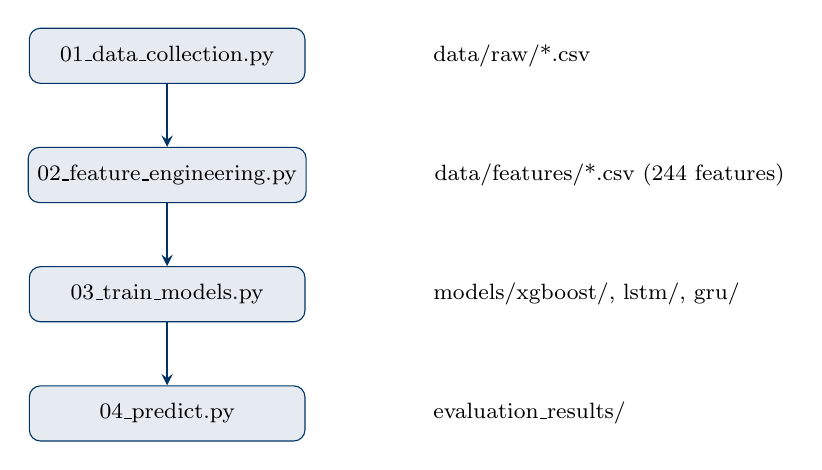
\begin{tikzpicture}[
        node distance=0.8cm,
        box/.style={rectangle, draw=primaryblue, fill=primaryblue!10, minimum width=3.5cm, minimum height=0.7cm, align=center, rounded corners, font=\footnotesize},
        arrow/.style={->, >=stealth, thick, primaryblue}
    ]
        \node[box] (data) {01\_data\_collection.py};
        \node[box, below=of data] (feat) {02\_feature\_engineering.py};
        \node[box, below=of feat] (train) {03\_train\_models.py};
        \node[box, below=of train] (pred) {04\_predict.py};
        
        \node[right=1.5cm of data, font=\footnotesize] {data/raw/*.csv};
        \node[right=1.5cm of feat, font=\footnotesize] {data/features/*.csv (244 features)};
        \node[right=1.5cm of train, font=\footnotesize] {models/xgboost/, lstm/, gru/};
        \node[right=1.5cm of pred, font=\footnotesize] {evaluation\_results/};
        
        \draw[arrow] (data) -- (feat);
        \draw[arrow] (feat) -- (train);
        \draw[arrow] (train) -- (pred);
    \end{tikzpicture}
    \end{center}
    
    \begin{block}{Automated Pipeline}
        \texttt{python main\_pipeline.py --symbol RELIANCE --steps 1 2 3 4}
    \end{block}
\end{frame}

% ============================================================================
\section*{References}
% ============================================================================

\begin{frame}{References}
    \footnotesize
    \textbf{Academic Papers:}
    \begin{enumerate}
        \item Shah, D. et al. (2021). ``Stock Market Prediction Using Bi-LSTM.'' \textit{IEEE Access}.\\
              \textcolor{primaryblue}{\url{https://ieeexplore.ieee.org/document/9395265}}
        \item Shrivastav, S. \& Kumar, S. (2022). ``Comparison of RF and GBM for Stock Prediction.'' \textit{Journal of King Saud University}.\\
              \textcolor{primaryblue}{\url{https://www.sciencedirect.com/journal/journal-of-king-saud-university-computer-and-information-sciences}}
        \item Chen, T. \& Guestrin, C. (2016). ``XGBoost: A Scalable Tree Boosting System.'' \textit{KDD '16}.\\
              \textcolor{primaryblue}{\url{https://arxiv.org/abs/1603.02754}}
        \item Hochreiter, S. \& Schmidhuber, J. (1997). ``Long Short-Term Memory.'' \textit{Neural Computation}.\\
              \textcolor{primaryblue}{\url{https://www.bioinf.jku.at/publications/older/2604.pdf}}
    \end{enumerate}
    
    \vspace{0.3cm}
    \textbf{Libraries \& Tools:}
    \begin{itemize}
        \item \textbf{yfinance}: \textcolor{primaryblue}{\url{https://pypi.org/project/yfinance/}}
        \item \textbf{XGBoost}: \textcolor{primaryblue}{\url{https://xgboost.readthedocs.io/}}
        \item \textbf{TensorFlow/Keras}: \textcolor{primaryblue}{\url{https://www.tensorflow.org/}}
        \item \textbf{Scikit-learn}: \textcolor{primaryblue}{\url{https://scikit-learn.org/}}
    \end{itemize}
\end{frame}

\begin{frame}{References (Continued)}
    \footnotesize
    \textbf{Technical Indicators:}
    \begin{enumerate}
        \item Wilder, J.W. (1978). ``New Concepts in Technical Trading Systems.'' --- RSI, ATR, ADX\\
              \textcolor{primaryblue}{\url{https://www.amazon.com/New-Concepts-Technical-Trading-Systems/dp/0894590278}}
        \item Bollinger, J. (2002). ``Bollinger on Bollinger Bands.'' --- Bollinger Bands\\
              \textcolor{primaryblue}{\url{https://www.bollingerbands.com/}}
        \item Appel, G. (2005). ``Technical Analysis: Power Tools for Active Investors.'' --- MACD\\
              \textcolor{primaryblue}{\url{https://www.investopedia.com/terms/m/macd.asp}}
    \end{enumerate}
    
    \vspace{0.3cm}
    \textbf{Data Sources:}
    \begin{itemize}
        \item \textbf{Yahoo Finance}: \textcolor{primaryblue}{\url{https://finance.yahoo.com/}}
        \item \textbf{NSE India}: \textcolor{primaryblue}{\url{https://www.nseindia.com/}}
        \item \textbf{India VIX}: \textcolor{primaryblue}{\url{https://www.nseindia.com/products/content/equities/indices/india_vix.htm}}
    \end{itemize}
    
    \vspace{0.3cm}
    \textbf{Future Work - API:}
    \begin{itemize}
        \item \textbf{AngelOne SmartAPI}: \textcolor{primaryblue}{\url{https://smartapi.angelbroking.com/docs}}
    \end{itemize}
\end{frame}

% ============================================================================
% THANK YOU SLIDE
% ============================================================================

\begin{frame}
    \begin{center}
        \Huge \textbf{Thank You!}
        
        \vspace{1cm}
        \Large Questions?
        
        \vspace{1cm}
        \normalsize
        \textbf{Vishwam Shah}\\
        Under the Guidance of Dr. Jigarkumar Shah\\
        Pandit Deendayal Energy University
        
        \vspace{0.5cm}
        \textcolor{primaryblue}{December 2025}
    \end{center}
\end{frame}

\end{document}
